\documentclass[12pt,paper=a4,twoside]{scrartcl}
\usepackage[T1]{fontenc}
\usepackage[utf8]{inputenc}
\usepackage{ae,aecompl}
\usepackage{amsmath}
\usepackage{graphicx}
\usepackage{color}
%\usepackage{xcolor}
\usepackage{epstopdf}
\usepackage{url}
%\usepackage{bbm}
\usepackage{listings}
\usepackage[font=small,labelfont=bf]{caption}
\usepackage[hidelinks]{hyperref}
\usepackage{booktabs}
\usepackage{pdfpages}
%\usepackage{bbold}
\usepackage[english]{babel}
\usepackage{amssymb}
%\usepackage{dsfont}
\usepackage{physics}
\usepackage{subcaption}
\usepackage{siunitx}
\usepackage{tabularx,multirow}
\sisetup{output-exponent-marker=\ensuremath{\mathrm{e}}}
%\usepackage[showframe]{geometry}
\numberwithin{equation}{section}
%\numberwithin{figure}{section}
\usepackage{listings}
%\usepackage{biblatex}

\usepackage{datatool}
\DTLsetseparator{ = }
\usepackage{pgf}

\usepackage[
backend=bibtex,
sorting=none,
style=numeric,
url=false,
giveninits
]{biblatex}
% Suppress month, number. 
\AtEveryBibitem{%
  \clearfield{month}%
}
% Don't do anything weird with journal name (default is italics).
\DeclareFieldFormat{journaltitle}{#1}
% Don't do anything weird with pages (default has pp in front).
\DeclareFieldFormat{pages}{#1}
% This block of code determines what kinds of fields you want in your
% bibliography entry, and it determines the order.
\DeclareBibliographyDriver{article}{%
  \usebibmacro{author/translator+others}%
  \addperiod\space
  \usebibmacro{title}%
  \usebibmacro{journal}%
  \addcomma
  \usebibmacro{volume+number+eid}%
  \usebibmacro{note+pages}%
  \usebibmacro{issue+date}%
  \usebibmacro{doi+eprint+url}%
  \usebibmacro{finentry}}

%\addbibresource{Literatur.bib}

\makeindex

\newcommand{\minus}{\scalebox{0.7}[0.9]{$-$}}
\newcommand{\mal}{\scalebox{0.7}[0.9]{$\cdot$}}
\newcommand{\rsmear}{r_\text{smear}}
%\DeclareMathOperator{\Tr}{Tr}
\renewcommand{\Re}{\mathop{\mathrm{Re}}}
\newcommand{\id}{{\mathbf 1}}


\usepackage{wrapfig}
\def\abs{\@ifstar{\oldabs}{\oldabs*}}

\definecolor{DARKbackcolour}{rgb}{0.16,0.17,0.2}
\definecolor{DARKcodecolor}{rgb}{0.67,0.70,0.75}
\definecolor{DARKnumbersgray}{rgb}{0.29,0.33,0.39}
\definecolor{DARKcodepurple}{rgb}{0.33,0.71,0.76}
\definecolor{DARKstringcolor}{rgb}{0.54,0.73,0.47}
\definecolor{DARKcommentcolor}{rgb}{0.36,0.39,0.41}

\definecolor{WHITEbackcolour}{rgb}{0.98,0.98,0.98}
\definecolor{WHITEcodecolor}{rgb}{0.22,0.23,0.26}
\definecolor{WHITEnumbersgray}{rgb}{0.76,0.76,0.76}
\definecolor{WHITEcodepurple}{rgb}{0.65,0.15,0.64}
\definecolor{WHITEstringcolor}{rgb}{0.31,0.63,0.31}
\definecolor{WHITEcommentcolor}{rgb}{0.63,0.63,0.65}

\lstdefinestyle{dark}{
    backgroundcolor=\color{DARKbackcolour},   
    numbers=left,
    numberstyle=\color{black},
    basicstyle=\color{DARKcodecolor}\ttfamily\small,
    keywordstyle=\color{DARKcodepurple},
    stringstyle=\color{DARKstringcolor},
    breaklines=true,
    tabsize=2,
    commentstyle=\color{DARKcommentcolor},
    captionpos=b,
    showspaces=false,
    showtabs=false
}
\lstdefinestyle{white}{
    backgroundcolor=\color{WHITEbackcolour},   
    %numbers=left,
    numberstyle=\color{black},
    basicstyle=\color{WHITEcodecolor}\ttfamily\small,
    keywordstyle=\color{WHITEcodepurple},
    stringstyle=\color{WHITEstringcolor},
    breaklines=true,
    tabsize=2,
    commentstyle=\color{WHITEcommentcolor},
    captionpos=b,
    showspaces=false,
    showtabs=false
}

\lstset{style=dark}

\begin{document}


\DTLloaddb[noheader, keys={thekey,thevalue}]{mydata}{snipets_data.dat}
\newcommand{\loadVOne}[1]{\DTLgetvalueforkey{\dataValueOne}{thevalue}{mydata}{thekey}{#1}}
\newcommand{\loadVTwo}[1]{\DTLgetvalueforkey{\dataValueTwo}{thevalue}{mydata}{thekey}{#1}}


\vspace*{1cm}
\Large
\begin{center}
PiADC Project
\end{center}
\vspace{3mm}
\normalsize
\begin{center}
Bent Buttwill
\end{center}
\vspace{2cm}
%\tableofcontents
\section{Introduction}
The goal of this project is to get used to the environment the Raspberry Pi brings along. With this in mind the project uses almost all of the topics taught in the lecture "Data Systems for Experimental Physics" PHYS391 UiB. 

One simple use case for the Raspberry Pi, hereafter named RPi, with its 40 GPIO (General-purpose input/output) pins, is to use it as a data acquisition device.
 Although none the its pins can read analog signals, in connection with an ADC chip (Analog-digital converter) one can add this function to its repertoire. 
To communicate with the ADC chip the RPi can take advantage of its SPI (Serial Peripheral Interface) pins. Together with its networking abilities the RPi can be used for data acquisition in physical experiments or for home automation.
\vspace{5mm}\\
The project will include 3 binary files compiled from C. Two of which will be running on the RPi and one on a PC. The structure is represented in Fig.~\ref{schematic}. As one can see on the RPi and and the PC there are programs running which are establishing the networking between each other. This is done by using sockets.
\vspace{10mm}\\

\section{Socket connection}
The server side is running on the RPi and uses the following code to open a socket and wait for a client to connect. The execution of the program will halt in line 16 and will continue after a client wants to connect. It is important to note that the server as well as the client are using the same byte order. For example the value for \verb+server_address.sin_port+ was given in network byte order. The function \verb+htons()+ turns the bytes from host into network byte order. This has to be done on both sides, so that both machines read the port number in the same way.

\loadVOne{ServerSocketB}
\loadVTwo{ServerSocketE}
\lstinputlisting[language=C, firstnumber={\dataValueOne}, firstline={\dataValueOne}, lastline={\dataValueTwo},caption=Server side socket initialization.]{../pi.c}

The client side tries to establish connect with the server. Upon successful connection the rest of the code will be executed.
\loadVOne{ClientSocketB}
\loadVTwo{ClientSocketE}
\lstinputlisting[language=C, firstnumber={\dataValueOne}, firstline={\dataValueOne}, lastline={\dataValueTwo},caption=Client side socket initialization.]{../pc.c}

After successful connecting both the server and the client will start their send and receive threads and will then be trapped in infinite loops.

\loadVOne{ClientStartThreadB}
\loadVTwo{ClientStartThreadE}
\lstinputlisting[language=C, firstnumber={\dataValueOne}, firstline={\dataValueOne}, lastline={\dataValueTwo},caption=Client starting send/recieve threads and sitting endlessly in for-loop\text{,} waiting for input of user.]{../pc.c}
The if-ladder included in the endless for-loop is responsible for interpreting the input of the user in the shell console. If the input is "s" it will change the \verb+sendState+ to 1 and will therefore send a signal to the RPi, more on that later. If the user types in "p" and hits enter it will fork into a sub-process which will be running the \verb+Gnuplot+ script \verb+plot.p+. This will plot the last 10,000 lines from the output file and continuously refreshing the plot. Upon receiving "q" as an input the client will leave the endless loop and exit the process.

\loadVOne{ServerStartThreadB}
\loadVTwo{ServerStartThreadE}
\lstinputlisting[language=C, firstnumber={\dataValueOne}, firstline={\dataValueOne}, lastline={\dataValueTwo},caption=Server starting send/recieve threads and waiting in for-loop endlessly.]{../pi.c}
\section{Sending and receiving threads}
\subsection{Client side}
The receiving thread on the client is reading from the socket and storing the data in output file. The \verb+fflush(file)+ command is later important as it writes to the file without closing it.
\loadVOne{ClientRecievingThreadB}
\loadVTwo{ClientRecievingThreadE}
\lstinputlisting[language=C, firstnumber={\dataValueOne}, firstline={\dataValueOne}, lastline={\dataValueTwo},caption=Receiving thread on client.]{../pc.c}
The thread for sending a signal to the RPi loops indefinetly too and writes the letter $s$ to the socket when the \verb+sendState+ gets set to 0 from the \verb+main+.
\loadVOne{ClientSendingThreadB}
\loadVTwo{ClientSendingThreadE}
\lstinputlisting[language=C, firstnumber={\dataValueOne}, firstline={\dataValueOne}, lastline={\dataValueTwo},caption=Sending thread on client.]{../pc.c}
\subsection{Server side}
For the server the sending and receiving threads are some what more interesting.

The sending thread is reading the data from shared memory guided by semaphores, to ensure the accessing of the memory only happens one at a time.
\loadVOne{ServerSendingThreadB}
\loadVTwo{ServerSendingThreadE}
\lstinputlisting[language=C, firstnumber={\dataValueOne}, firstline={\dataValueOne}, lastline={\dataValueTwo},caption=Thread for reading from shared memory\text{,} sending to client.]{../pi.c}

After initialization of the shared memory and the semaphore in the first code block this thread also gets trapped in an endless for loop. The function \verb+semaphore_p()+ asks linux if it can access the shared memory and waits for approval. When this thread gets the token from the system the execution can continue. Then the data gets copied from the shared memory into the socket and then send to the PC. After sleeping for about 100$\mu s$ the semaphore gets released so that the other program can access the shared memory again.
The structure of the shared memory has to be exactly defined. This is done by calling the following.
\loadVOne{SharedMemoryStrucB}
\loadVTwo{SharedMemoryStrucE}
\lstinputlisting[language=C, firstnumber={\dataValueOne}, firstline={\dataValueOne}, lastline={\dataValueTwo},caption=The structure used for the shared memory.]{../dataAq.c}
\subsubsection{GPIO pins used by receiving thread}
The receiving part on the RPi is also running continuously and checks if the incoming character is correct. Upon recieval the LED on GPIO pin 5 turn on for 1 second.
\loadVOne{ServerRecievingThreadB}
\loadVTwo{ServerRecievingThreadE}
\lstinputlisting[language=C, firstnumber={\dataValueOne}, firstline={\dataValueOne}, lastline={\dataValueTwo},caption=Upon receiving the correct character the LED on GPIO pin 5 turns on for 1 second.]{../pi.c}
First the GPIO pins have to be configured. For this the addresses in memory are going to be mapped to virtual memory that is accessible for this program. This happens in the \verb+setup_io();+ function which is included in the \verb+GPIO.h+ header file. To put a specific GPIO pin into output mode one has to set it into input mode first and then into output mode. This is done via \verb+INP_GPIO(gpio_pin)+ and \verb+OUT_GPIO(gpio_pin)+ respectively. With the commands \verb+GPIO_SET = 1 << gpio_pin+ and \verb+GPIO_CLR = 1 << gpio_pin+ one can set the GPIO pin into the high and low state respectively. This is done by bit shifting a 1 bit to the correct position in memory.
\section{Data acquisition program}
In the program \verb+dataAq.c+ the interesting processing happens. This program doesn't use threads as its only purpose is to read out the ADC chip and write the data to the shared memory. The code obviously also uses the same semaphore and shared memory initializtaion as \verb+pi.c+ does, the interesting part of the code is the SPI usage. SPI is needed to have an easy way to talk to the ADC chip. SPI is a synchronous serial communication interface used to communicate with different microchips. It enables easy communication between different devices. It uses 4 lines to connect master with slave. One line $SCLK$ is used as a clock line, so that both devices are synced at the same frequency. Two lines $MOSI$ and $MISO$, master-out slave-in and master-in slave-out respectively, are used to enable the communication. The last line is used to select the corresponding SPI device. With SPI it is also possible to talk to more than one device on the same lines. For this the master either has multiple select lines or the SPI device are connected in series.

Before communicating with a device over SPI one has to specify the communication details.
For this one has to write into the \verb+spi_setting+ structure defined in the \verb+mcp3008.h+ header file.
\loadVOne{SPISettingB}
\loadVTwo{SPISettingE}
\lstinputlisting[language=C, firstnumber={\dataValueOne}, firstline={\dataValueOne}, lastline={\dataValueTwo},caption=Setting the SPI settings.]{../dataAq.c}

The RPi supports up to two SPI devices connected to its corresponding pins. To talk to the device connected to pin 24 corresponds one has to open the system file "/dev/spidev0.0", for devices connected to pin 26 one has to use "/dev/spidev1.0". This is done in the \verb+spiOpen()+ function. The rest of the SPI setting are specified by the device you are trying to connect to.

The actual communication with the SPI device is done by calling the \verb+spiWriteRead+ function. One has to give it a data array containing the information that one wants to send to the SPI device. In the same data array will be the data written that the SPI device sends back.
\loadVOne{ReadSPIdeviceB}
\loadVTwo{ReadSPIdeviceE}
\lstinputlisting[language=C, firstnumber={\dataValueOne}, firstline={\dataValueOne}, lastline={\dataValueTwo},caption=Reading the SPI device and writing to the shared memory.]{../dataAq.c}

\begin{figure}
\centering
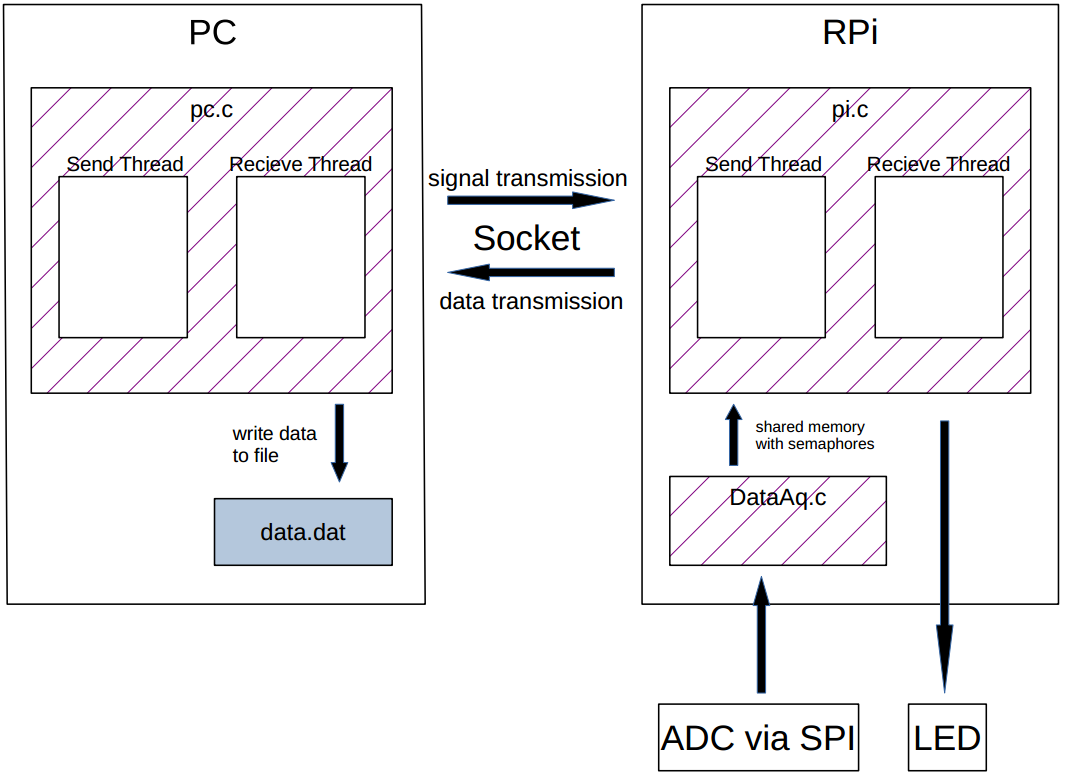
\includegraphics[scale=0.4]{schematic.png}
\caption{Structure of this project. Binary files are represented as hatched.}
\label{schematic}
\end{figure}

\end{document}
